\documentclass[aspectratio=169,12pt]{beamer}
\usetheme{Madrid}
\usecolortheme{dolphin}
\usefonttheme{professionalfonts}
\setbeamertemplate{navigation symbols}{}
\setbeamertemplate{footline}{}

\usepackage[T1]{fontenc}
\usepackage[utf8]{inputenc}
\usepackage{graphicx}
\usepackage{amsmath,amssymb}
\usepackage{hyperref}
\usepackage{siunitx}
\usepackage{physics}
\usepackage{braket}

\graphicspath{{../../figures/}}

\title[Module A5]{Module A5: Circuits et portes logiques}
\author{JAMOTTE Maxime, SCHOONEN Cédric}
\institute{Digital Learning Hub}
\date{}

\begin{document}

\begin{frame}
  \titlepage
\end{frame}

\begin{frame}{Objectifs du module A5}
  \begin{enumerate}
    \item Portes logiques classiques et circuits\\~\\
    \item Portes logiques quantiques sur 1 qubit: $X$, $Z$, $H$\\~\\
    \item Portes logiques quantiques sur 2 qubits: SWAP, CNOT, CZ\\~\\
    \item Génération des paires de Bell par circuit ($H$ + CNOT)\\~\\
    \item Représentation symbolique: circuits quantiques\\~\\
    \item Modèle de calcul: circuit $\rightarrow$ exécution sur QPU $\rightarrow$ résultats de mesures
  \end{enumerate}
\end{frame}

% ============================================================
\section{Portes logiques classiques}
% ============================================================

\begin{frame}{Portes logiques classiques}
  \begin{itemize}[<+->]
    \setlength{\itemsep}{0.55em}
    \item Bits classiques: 0 ou 1; les portes transforment ces bits.
    \item Exemples clés : NOT, AND, OR, XOR, NAND (porte universelle).
    \item On enchaîne ces portes pour construire des circuits logiques.
  \end{itemize}
  \vfill
  \only<2->{%
    \centering
    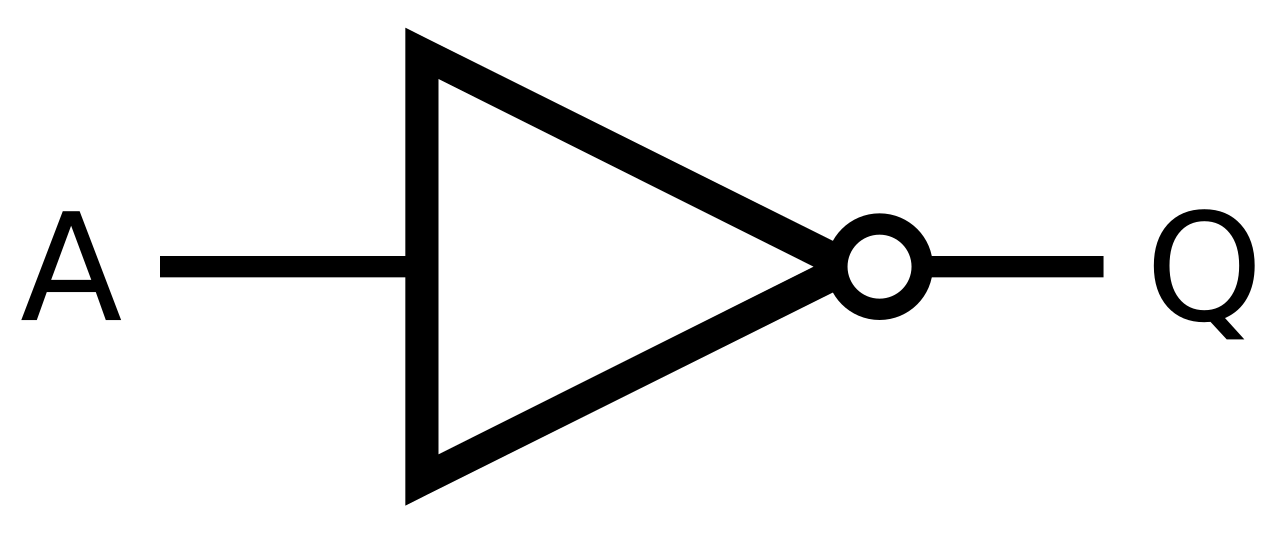
\includegraphics[height=1.1cm]{NOT.png}\hspace{0.3cm}
    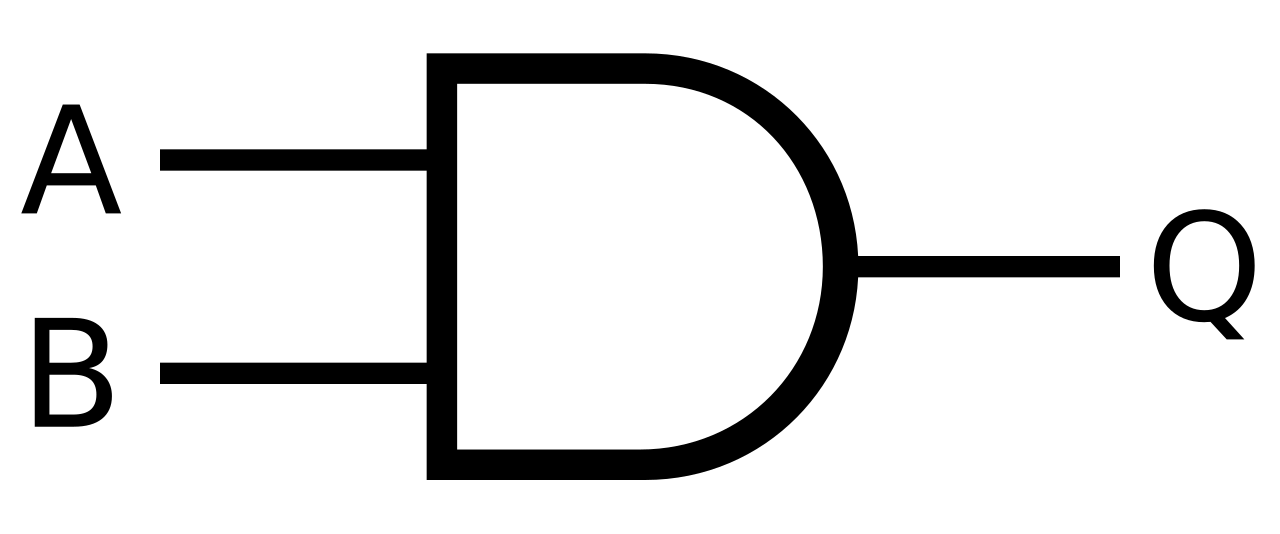
\includegraphics[height=1.1cm]{AND.png}\hspace{0.3cm}
    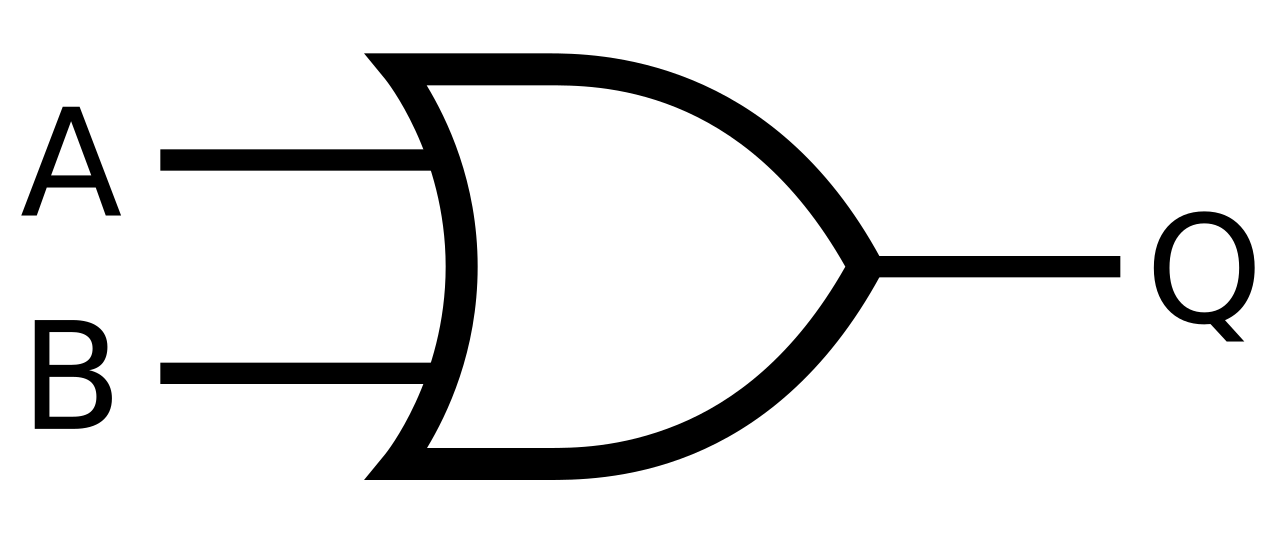
\includegraphics[height=1.1cm]{OR.png}\hspace{0.3cm}
    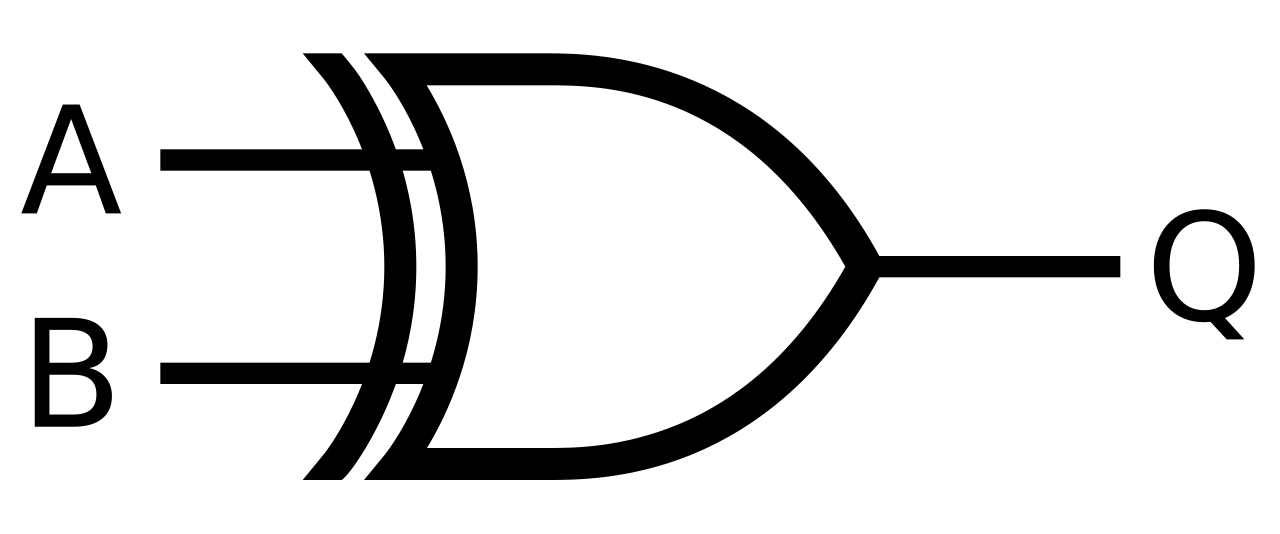
\includegraphics[height=1.1cm]{XOR.png}\hspace{0.3cm}
    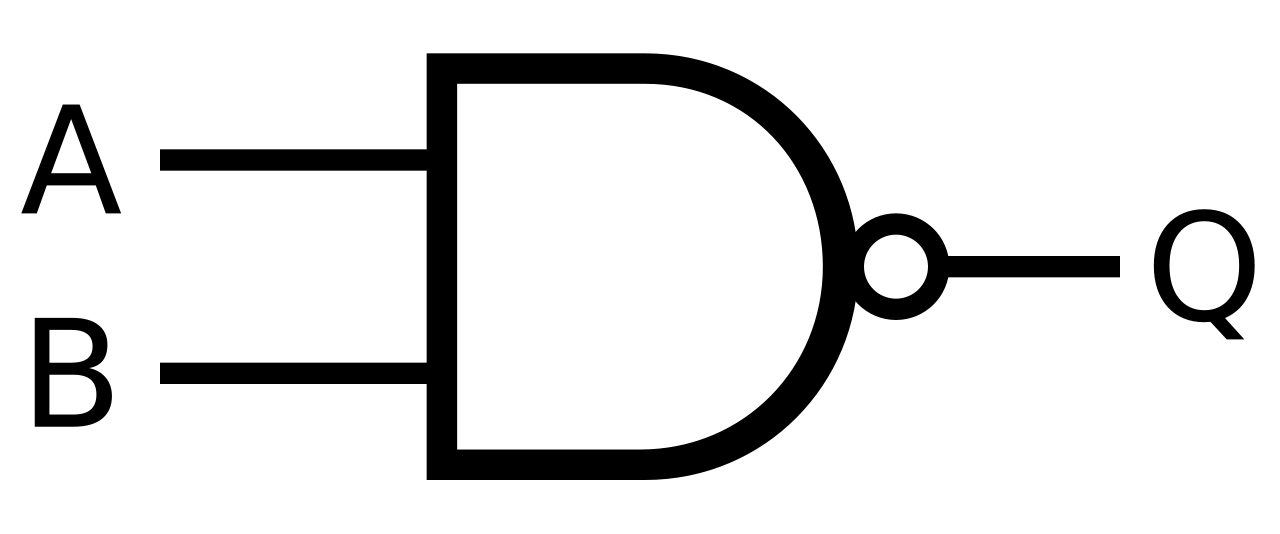
\includegraphics[height=1.1cm]{NAND.png}
  }
\end{frame}

\begin{frame}{Table de vérité (rappel)}
  \centering
  \renewcommand{\arraystretch}{1.4}
  \begin{tabular}{l c c c}
    \textbf{Porte} & \textbf{Symbole} & \textbf{Expression} & \textbf{Description} \\\hline
    NOT   & $\lnot A$ & inverse & $1\leftrightarrow 0$ \\
    AND   & $A\cdot B$ & $1$ si $A=1$ et $B=1$ & porte "multiplication" \\
    OR    & $A + B$ & $1$ si $A=1$ ou $B=1$ & porte "addition" \\
    XOR   & $A \oplus B$ & $1$ si $A\neq B$ & "ou exclusif" \\
    NAND  & $\lnot(A\cdot B)$ & inverse de AND & base universelle \\
  \end{tabular}
\end{frame}

\begin{frame}{Table de vérité XOR / AND}
  \centering
  \renewcommand{\arraystretch}{1.4}
  \begin{tabular}{c c | c | c}
    $A$ & $B$ & $A\ \mathbf{XOR}\ B$ & $A\ \mathbf{AND}\ B$ \\\hline
    0 & 0 & 0 & 0 \\
    0 & 1 & 1 & 0 \\
    1 & 0 & 1 & 0 \\
    1 & 1 & 0 & 1 \\
  \end{tabular}
\end{frame}

\begin{frame}{Exemple de circuit classique}
  \begin{itemize}[<+->]
    \item Enchaînement de portes pour additionner deux bits (avec report).
    \item Chaque fil transporte un bit, chaque symbole applique une porte.
  \end{itemize}
  \vfill
  \centering
  
\includegraphics[width=0.65\textwidth]{addition_circuit2.png}
\end{frame}

% ============================================================
\section{Portes logiques quantiques sur 1 qubit}
% ============================================================

\begin{frame}{Portes logiques quantiques}
  \begin{itemize}[<+->]
    \setlength{\itemsep}{0.6em}
    \item Les actions sur les qubits sont des \textbf{portes logiques quantiques}.\\~\\
    \item Toute transformation quantique est \textbf{réversible} (inversible).\\~\\
    \item Les portes logiques quantiques sont représentées par des \textbf{matrices unitaires}
     ($U^\dagger U = I$).
  \end{itemize}
\end{frame}

\begin{frame}{Porte $X$ (NOT quantique)}
  \begin{itemize}[<+->]
    \setlength{\itemsep}{0.55em}
    \item Matrice: $X = \begin{pmatrix} 0 & 1 \\ 1 & 0 \end{pmatrix}$\\~\\
    \item Action: $X\ket{0} = \ket{1}, \quad X\ket{1} = \ket{0}$.\\~\\
    \item Analogue quantique de la porte NOT classique:
     inverse les amplitudes de $\ket{0}$ et $\ket{1}$.
  \end{itemize}
\end{frame}

\begin{frame}{Porte $Z$}
  \begin{itemize}[<+->]
    \setlength{\itemsep}{0.55em}
    \item Matrice: $Z = \begin{pmatrix} 1 & 0 \\ 0 & -1 \end{pmatrix}$\\~\\
    \item Action: $Z\ket{0} = \ket{0}, \quad Z\ket{1} = -\ket{1}$.\\~\\
    \item Change le \textit{signe} (la phase) de $\ket{1}$ sans modifier les probabilités.
  \end{itemize}
\end{frame}

\begin{frame}{Porte de Hadamard $H$}
  \begin{itemize}[<+->]
    \setlength{\itemsep}{0.55em}
    \item Matrice: $H = \dfrac{1}{\sqrt{2}} \begin{pmatrix} 1 & 1 \\ 1 & -1 \end{pmatrix}$\\~\\
    \item Action:
    $$H\ket{0} = \frac{\ket{0}+\ket{1}}{\sqrt{2}} = \ket{+}, \qquad
      H\ket{1} = \frac{\ket{0}-\ket{1}}{\sqrt{2}} = \ket{-}.$$
    \item Crée une \textbf{superposition} à partir d'un état de base.
  \end{itemize}
\end{frame}

% ============================================================
\section{Portes logiques quantiques sur 2 qubits}
% ============================================================

\begin{frame}{Porte SWAP}
  \begin{itemize}[<+->]
    \setlength{\itemsep}{0.55em}
    \item Permute les deux qubits: $\text{SWAP}\ket{ab} = \ket{ba}$.\\~\\
    \item Matrice dans la base computationnelle $\{\ket{00},\ket{01},\ket{10},\ket{11}\}$:
    $$\text{SWAP} = \begin{pmatrix} 1&0&0&0 \\ 0&0&1&0 \\ 0&1&0&0 \\ 0&0&0&1 \end{pmatrix}$$
  \end{itemize}
\end{frame}

\begin{frame}{Porte CNOT (controlled-NOT)}
  \begin{columns}[T,onlytextwidth]
    \column{0.55\textwidth}
    \begin{itemize}[<+->]
      \setlength{\itemsep}{0.55em}
      \item Inverse le qubit \textbf{cible} si le qubit \textbf{contrôle} est $\ket{1}$.
      \item CNOT$\ket{00}=\ket{00}$, CNOT$\ket{01}=\ket{01}$,
       CNOT$\ket{10}=\ket{11}$, CNOT$\ket{11}=\ket{10}$.
      \item Matrice:
      $$\text{CNOT} = \begin{pmatrix} 1&0&0&0 \\ 0&1&0&0 \\ 0&0&0&1 \\ 0&0&1&0 \end{pmatrix}$$
    \end{itemize}
    \column{0.4\textwidth}
    \centering
    \includegraphics[width=0.7\linewidth]{CNOT.png}
    \\[0.3em]\footnotesize Symbole du CNOT
  \end{columns}
\end{frame}

\begin{frame}{Porte CZ (controlled-Z)}
  \begin{itemize}[<+->]
    \setlength{\itemsep}{0.55em}
    \item Applique $Z$ au qubit cible si le qubit contrôle est $\ket{1}$:
     CZ$\ket{11} = -\ket{11}$.\\~\\
    \item Matrice:
    $$\text{CZ} = \begin{pmatrix} 1&0&0&0 \\ 0&1&0&0 \\ 0&0&1&0 \\ 0&0&0&-1 \end{pmatrix}$$
    \item La porte CZ est \textbf{symétrique}: peu importe quel qubit est le contrôle.
  \end{itemize}
\end{frame}

\begin{frame}{Hadamard en parallèle}
  \begin{itemize}[<+->]
    \setlength{\itemsep}{0.55em}
    \item Pour appliquer $H$ à chaque qubit indépendamment, on utilise $H\otimes H$:
    $$(H\otimes H)\ket{00} = H\ket{0}\otimes H\ket{0}
     = \frac{\ket{0}+\ket{1}}{\sqrt{2}}\otimes\frac{\ket{0}+\ket{1}}{\sqrt{2}}$$
    $$= \frac{1}{2}\big(\ket{00}+\ket{01}+\ket{10}+\ket{11}\big)$$
    \item Superposition \textbf{uniforme} sur les 4 états de base.
  \end{itemize}
\end{frame}

\begin{frame}{Génération des paires de Bell}
  \begin{columns}[T,onlytextwidth]
    \column{0.55\textwidth}
    \begin{itemize}[<+->]
      \setlength{\itemsep}{0.55em}
      \item Appliquer $H$ sur le premier qubit puis CNOT:
      $$\ket{00} \xrightarrow{H\otimes I} \frac{\ket{0}+\ket{1}}{\sqrt{2}}\ket{0}$$
      $$\xrightarrow{\text{CNOT}} \frac{\ket{00}+\ket{11}}{\sqrt{2}} = \ket{\Phi^+}$$
      \item C'est un état \textbf{intriqué}: la paire de Bell $\ket{\Phi^+}$.
    \end{itemize}
    \column{0.4\textwidth}
    \centering
    \includegraphics[width=0.85\linewidth]{bell_pair_circuit.png}
    \\[0.3em]\footnotesize Circuit de paire de Bell
  \end{columns}
\end{frame}

\begin{frame}{Mesures sur les paires de Bell}
  \begin{itemize}[<+->]
    \setlength{\itemsep}{0.55em}
    \item $\ket{\Phi^+} = \frac{1}{\sqrt{2}}(\ket{00}+\ket{11})$:\\
     mesurer le premier qubit donne $\ket{0}$ ou $\ket{1}$ avec probabilité $\frac{1}{2}$ chacun.\\~\\
    \item Si le premier qubit donne $\ket{0}$, le second est \textbf{nécessairement} $\ket{0}$ (et vice versa).\\~\\
    \item Les résultats sont toujours \textbf{parfaitement corrélés}, quelle que soit la distance entre les deux qubits.
  \end{itemize}
\end{frame}

% ============================================================
\section{Circuits quantiques}
% ============================================================

\begin{frame}{Représentation symbolique d'un calcul sur QPU}
  \begin{itemize}[<+->]
    \setlength{\itemsep}{0.55em}
    \item Les qubits se transforment via des portes logiques quantiques.\\~\\
    \item Les \textbf{vecteurs} représentant les \textbf{qubits} sont transformés par des \textbf{matrices}
     représentant les \textbf{portes quantiques}.\\~\\
    \item Les circuits quantiques enchaînent ces portes sur des lignes de qubits (analogie classique).
  \end{itemize}
\end{frame}

\begin{frame}{Le circuit décrit un état quantique}
  \begin{itemize}[<+->]
    \setlength{\itemsep}{0.55em}
    \item Tout circuit quantique part de l'état initial $\ket{00\cdots0}$.\\~\\
    \item La séquence de portes quantiques dans le circuit décrit la \textbf{construction} d'un état quantique.\\~\\
    \item Chaque porte agit sur un ou plusieurs qubits et modifie l'état global du système.
  \end{itemize}
\end{frame}

\begin{frame}{Modèle de calcul quantique}
  \begin{itemize}[<+->]
    \setlength{\itemsep}{0.55em}
    \item \textbf{Étape 1}: Construire le circuit (séquence de portes quantiques).\\~\\
    \item \textbf{Étape 2}: Exécuter le circuit sur un QPU (processeur quantique) ou un simulateur.\\~\\
    \item \textbf{Étape 3}: Mesurer les qubits et collecter les résultats.\\~\\
    \item L'exécution est répétée un certain nombre de fois (\textit{shots}) pour obtenir des statistiques sur les résultats de mesure.
  \end{itemize}
\end{frame}

\begin{frame}{Portes quantiques dans les circuits}
  \begin{columns}[T,onlytextwidth]
    \column{0.5\textwidth}
    \centering
    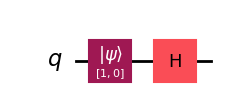
\includegraphics[width=0.75\linewidth]{gate_hadamard.png}
    \\[-0.3em]\footnotesize Circuit Qiskit pour $H$
    \column{0.5\textwidth}
    \centering
    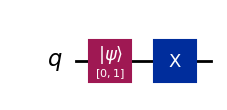
\includegraphics[width=0.75\linewidth]{gate_x.png}
    \\[-0.3em]\footnotesize Circuit Qiskit pour $X$
  \end{columns}
  ~\\~\\
  \begin{columns}[T,onlytextwidth]
    \column{0.5\textwidth}
    \centering
    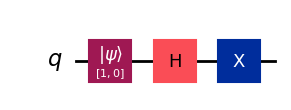
\includegraphics[width=0.75\linewidth]{gate_h_then_x.png}
    \\[-0.3em]\footnotesize Circuit $H$ puis $X$
    \column{0.5\textwidth}
    \centering
    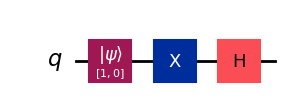
\includegraphics[width=0.75\linewidth]{gate_x_then_h.png}
    \\[-0.3em]\footnotesize Circuit $X$ puis $H$
  \end{columns}
\end{frame}

\begin{frame}{Circuit de mesure}
  \begin{columns}[T,onlytextwidth]
    \column{0.5\textwidth}
    \begin{itemize}
      \item Ajouter un bit classique pour stocker la mesure.
      \item Opération de mesure et stockage dans le bit classique.
      \item Probabilités obtenues par le module carré des amplitudes.
    \end{itemize}
    \column{0.45\textwidth}
    \centering
    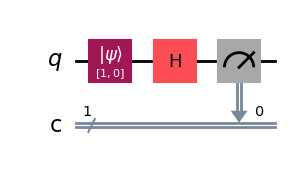
\includegraphics[width=0.9\linewidth]{measure_circuit.png}
  \end{columns}
\end{frame}

\begin{frame}{Fin du module A5}
  \centering
  \vfill
  Passons à la pratique avec Qiskit!
  \vfill
\end{frame}

\end{document}
